\documentclass[titlepage,dvipdfmx]{jsarticle}
\usepackage[final,hiresbb]{graphicx}
\usepackage{amsmath,amssymb}
\usepackage{amsfonts}
\usepackage{bm}
\begin{document}
\section{境界条件の物理的意味}
\subsection{熱伝導方程式で考えると}
$0{}^\circ $C の温度に保たれていた一辺が$L$の立方体の形をした熱伝導体を時刻$t=0$に温度$T_0 {}^\circ $Cのお湯に浸した。熱伝導体内部の温度分布$T$を決定せよ.\\
式は
\begin{equation}\displaystyle
\displaystyle \frac{\partial T}{\partial t}=\kappa  \frac{\partial^2 T}{\partial x^2} \nonumber
\end{equation}
となる(一次元方向のみ考える)
\subsubsection{熱が自由に出入りする場合$\rightarrow$温度一定、温度の出入り自由}

\begin{minipage}{.40\textwidth}
\flushleft
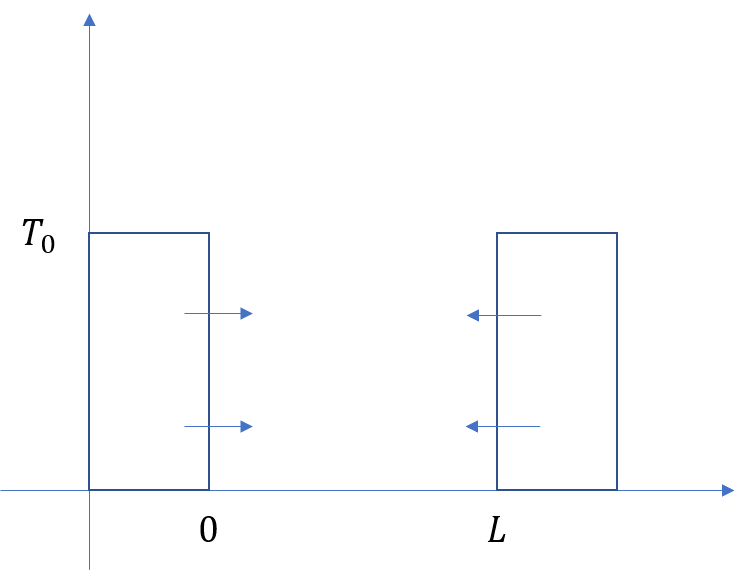
\includegraphics[height=4.5cm, clip]{1.png}
\end{minipage}
\hfill
\begin{minipage}{.50\textwidth}
$t\rightarrow \infty$で熱浴(周りのお湯)の温度に一致\\
\end{minipage}\\

\begin{minipage}{.40\textwidth}
\flushleft
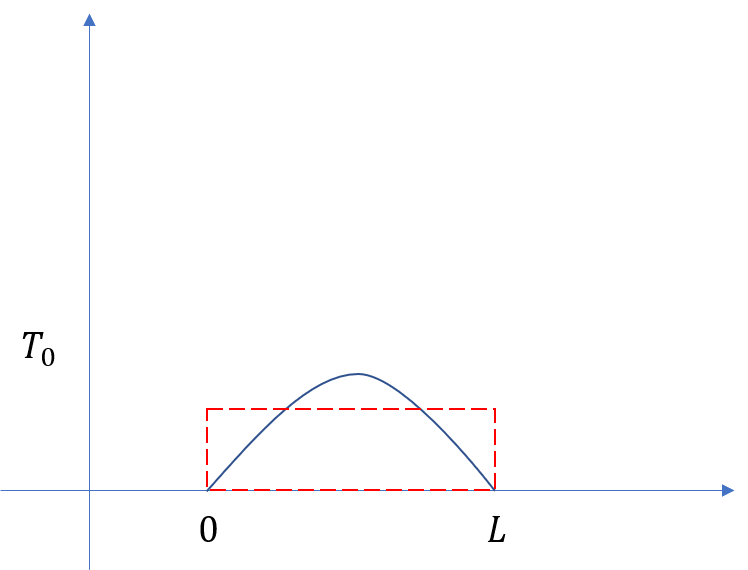
\includegraphics[height=4.5cm, clip]{2.png}
\end{minipage}
\hfill
\begin{minipage}{.50\textwidth}
断熱変化のため温度の流れがない、$\rightarrow$ 傾きがない
$\displaystyle \frac{\partial T}{\partial x}|_{x=0}=0,\frac{\partial T}{\partial x}|_{x=L}=0$
\end{minipage}\\
\subsubsection*{補足:もし一方が断熱もう一方が熱浴なら?}
一方(熱浴側)から熱の出入りが起こる
\subsection{計算をする前に...}
境界条件は扱いやすい(計算しやすい...0とか)形に!!
\subsubsection*{条件} \noindent
表面:$x=0,L$で$T(0,t)=T(L,t)=T_0~~~~\Rightarrow \widetilde{T}(x,t)=T(x,t)-T_0$とすると...\\
$\widetilde{T}(0,t)=\widetilde{T}(L,t)=0,\widetilde{T}(x,0)=-T_0$\\\\
方程式は変わらず
\begin{equation}\displaystyle
\displaystyle \frac{\partial \widetilde{T}}{\partial t}=\kappa  \frac{\partial^2 \widetilde{T}}{\partial x^2} \nonumber
\end{equation}
\subsection*{解法}
\noindent step1: 解を変数分離して代入\\
$\widetilde{T}= F(x)\cdot G(t)$\\
$\displaystyle \rightarrow F \cdot \frac{d G}{dt}=\kappa \frac{d^2 F}{d x^2}G$\\\\
step2:$(一変数のみの関数)=(違う文字の一変数のみの関数)$にする\\
$\displaystyle \Leftrightarrow \frac{1}{\kappa G}\cdot \frac{d G}{dt}= \frac{1}{F}\cdot \frac{d^2 F}{dx^2}$\\\\
step3: $(変数)=(変数)$と恒常的になるため(変数)$=$定数$k$とする\\
$\displaystyle \rightarrow \frac{d^2 F}{dx^2}=kF , \frac{dG}{dt}=\kappa k G$\\\\
step4: 2つの常微分方程式において解を求める(簡単なほうから)
$\displaystyle \frac{dG}{dt} =\kappa k G \rightarrow \therefore G =Ae^{\kappa k t}$\\
\begin{center}
$G\rightarrow (t\rightarrow \infty)は違うからk<0$ ここで$k=-l^2$
\end{center}
$\therefore F(x)=C_1\sin lx +C_2 \cos lx $ \\\\
境界条件 $\widetilde{T}(0,t)=\widetilde{T}(L,t)=0$から~~~~~~~~
$\displaystyle F(x)=C_1 \sin \frac{n\pi}{L}x$\\\\
規格化すると...~$\displaystyle F(x)=\sqrt{\frac{2}{L}}\cdot \sin \frac{n\pi}{L}x$
step5: 重ね合わせの原理を用いて解を表し、級数展開の要領で解く\\\\
\begin{equation}\displaystyle
\widetilde{T}=\sum_{n=1}^{\infty} c_n \sqrt{\frac{2}{L}} \sin \frac{n\pi}{L}x \cdot e^{-\kappa (\frac{n \pi }{L})^2t}
\nonumber
\end{equation}
初期条件から\\
\begin{equation}\displaystyle
-T_0=\sum_{n=1}^{\infty} c_n \sqrt{\frac{2}{L}} \sin \frac{n\pi}{L}x
\nonumber
\end{equation}
両辺に$\displaystyle \sqrt{\frac{2}{L}}\cdot \sin \frac{m\pi}{L}x$をかけて$0\rightarrow L$で$x$で積分すると、\\
$\displaystyle (左辺)=-T_0 \int_{0}^{L}\sqrt{\frac{2}{L}}\cdot \sin \frac{m\pi}{L}x dx=...=T_0 \sqrt{\frac{2}{L}}\cdot \frac{L}{n\pi}\left( \cos n\pi -1 \right)$\\
$\displaystyle (右辺)=c_n$\\
$~~\displaystyle ~~~~~~~~~~~~\rightarrow \widetilde{T}=-T_0 \sum_{m:奇数}^{\infty} 2T_0 \sqrt{\frac{2}{L}}\cdot \frac{L}{m\pi}\sqrt{\frac{2}{L}}\cdot \sin \frac{m\pi}{L}x \cdot e^{-\kappa \left(\frac{m\pi}{L}\right)^2 t}$\\
よって\\
\begin{equation}
\displaystyle
T(x,t)=T_0-\sum_{m:奇数}^{\infty} \frac {4T_0}{m\pi} \sin{\frac{m\pi}{L}}\cdot e^{-\kappa \left(\frac{m\pi}{L}\right)t}
\nonumber
\end{equation}
\subsubsection*{結果の意味}
徐々に温度が上がり、最終的には周囲の温度と一致する!


\end{document}
